\documentclass[a4paper,11pt]{article}
\input{/home/tof/Documents/Cozy/latex-include/preambule_lua.tex}
\newcommand{\showprof}{show them}  % comment this line if you don't want to see todo environment
\fancyhead[L]{Page web - spécialités}
\newdate{madate}{10}{09}{2020}
%\fancyhead[R]{\displaydate{madate}} %\today
%\fancyhead[R]{Seconde - SNT}
\fancyhead[R]{Première - NSI}
%\fancyhead[R]{Terminale - NSI}
\fancyfoot[L]{~\\Christophe Viroulaud}
\AtEndDocument{\label{lastpage}}
\fancyfoot[C]{\textbf{Page \thepage/\pageref{lastpage}}}
\fancyfoot[R]{\includegraphics[width=2cm,align=t]{/home/tof/Documents/Cozy/latex-include/cc.png}}

\begin{document}
\begin{Form}
\section{Problématique}
Pour aider les élèves de seconde dans leur orientation, le lycée décide de mettre en place une page web présentant les différentes spécialités enseignées en classe de première (figure \ref{pageweb}).
\begin{figure}[!h]
\centering
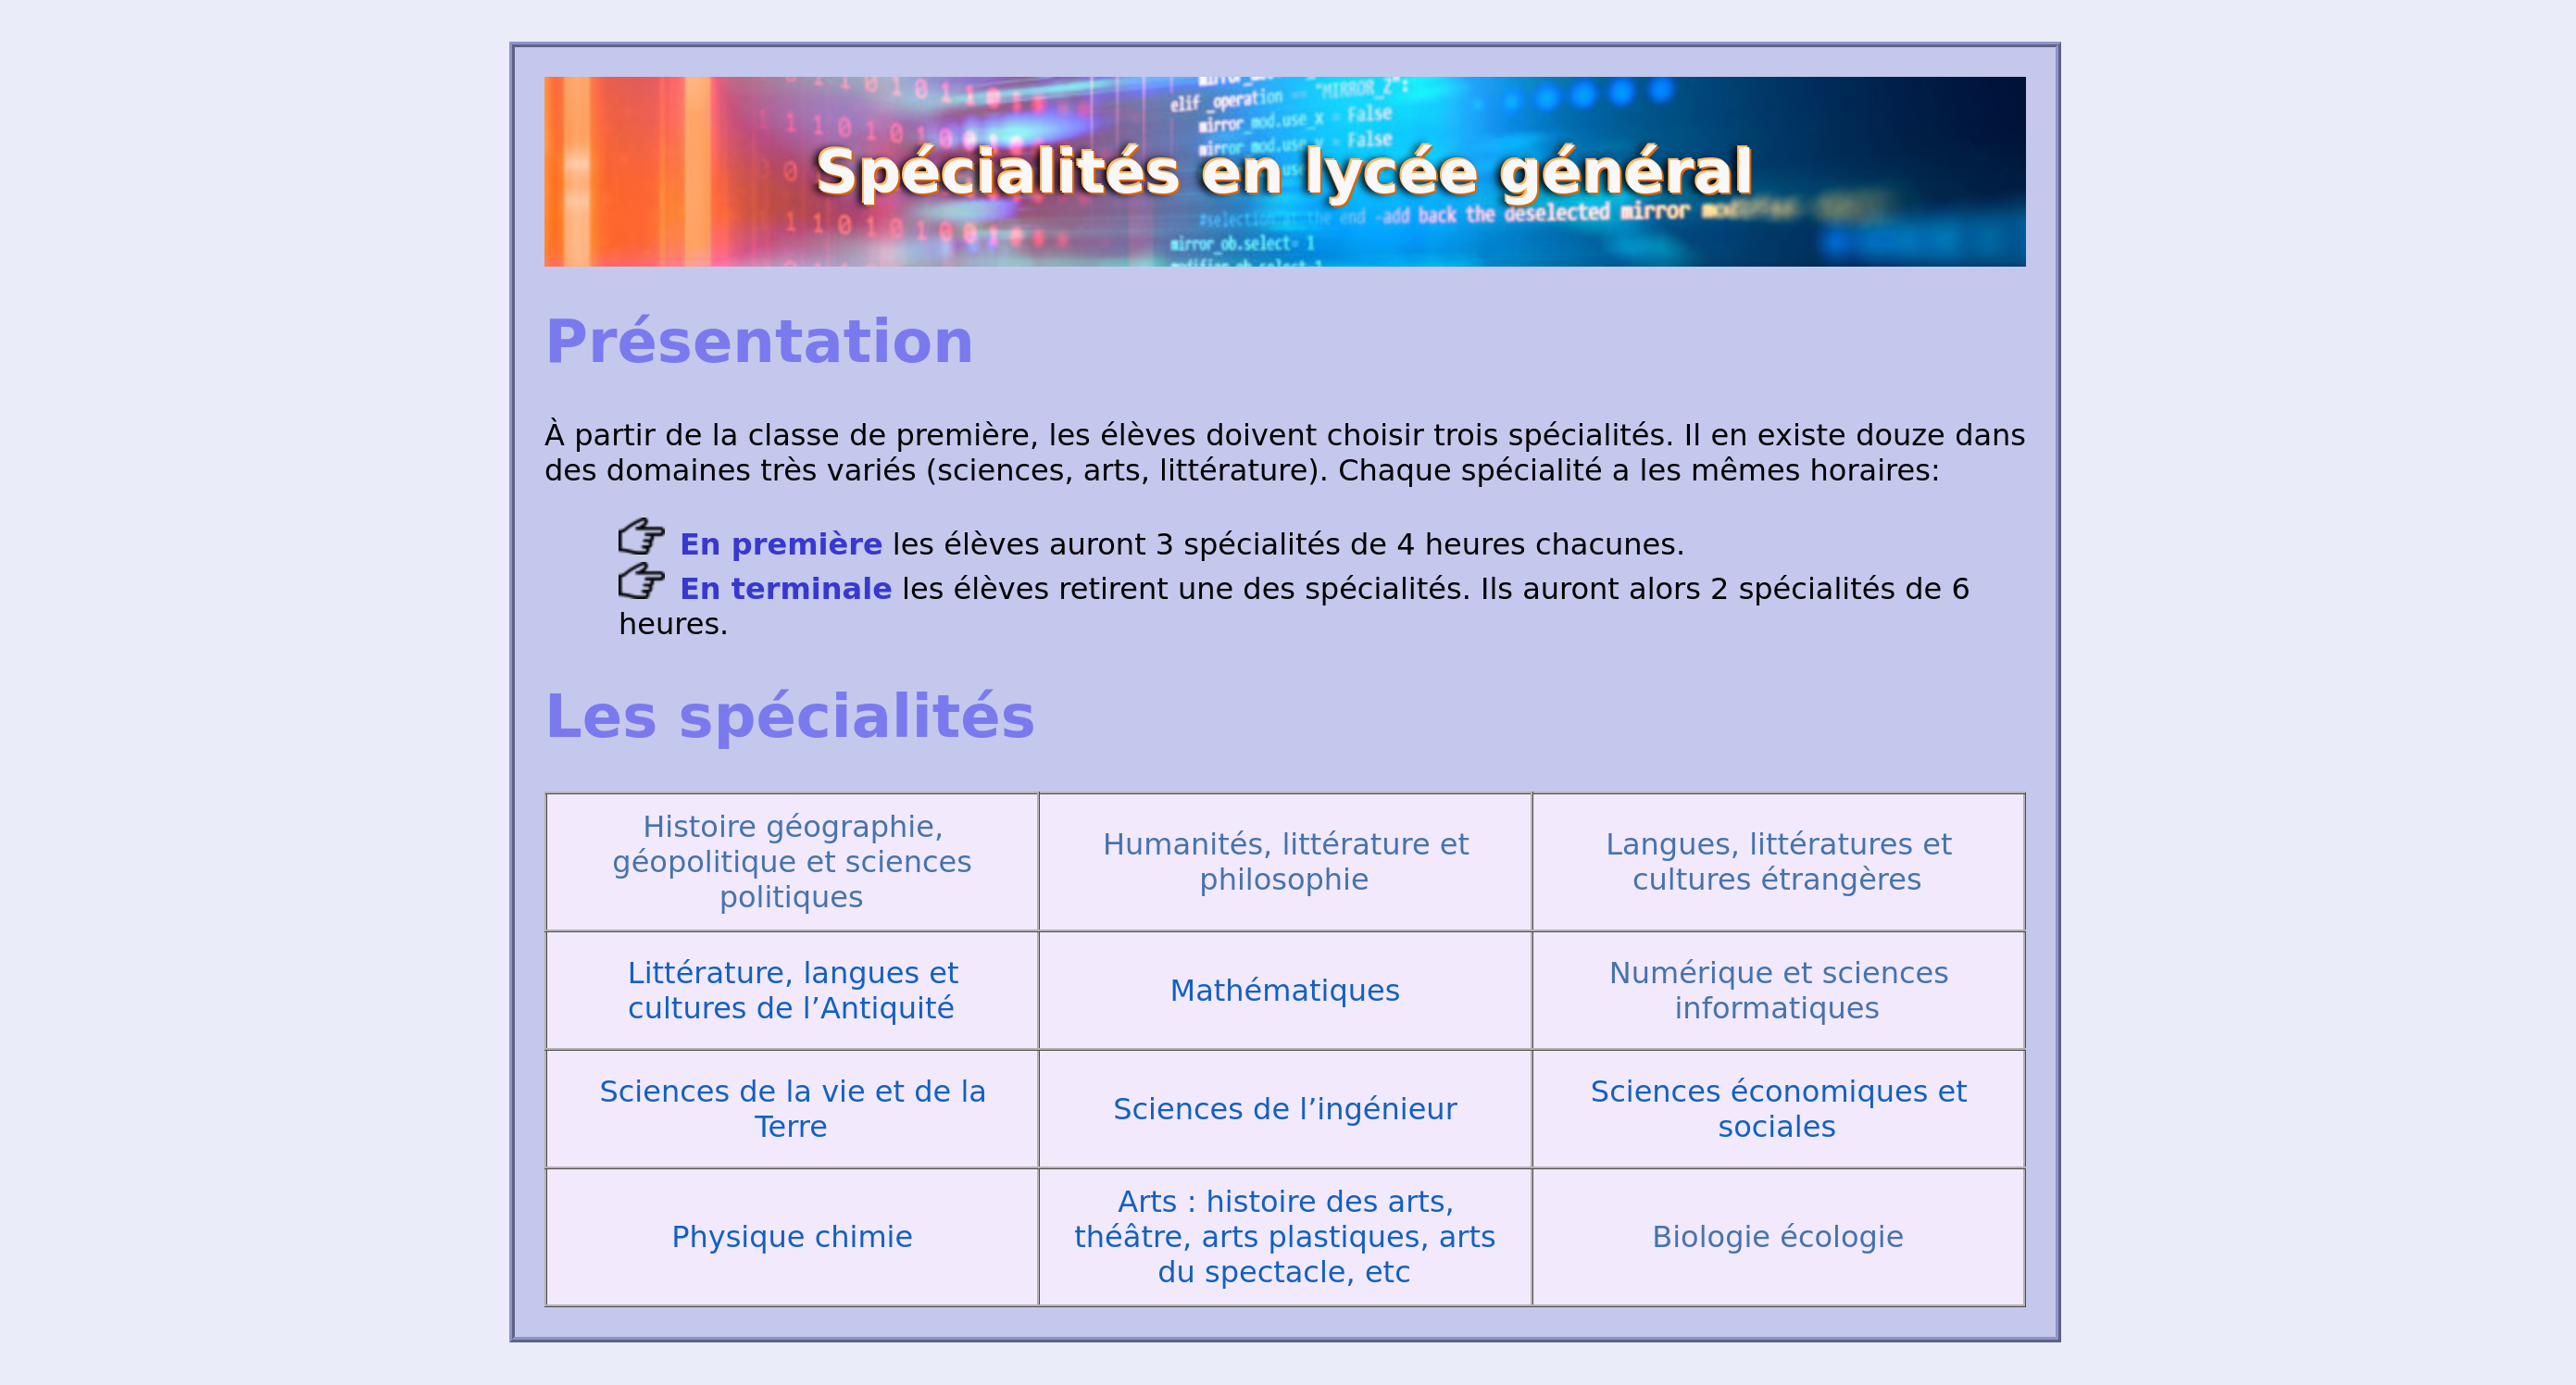
\includegraphics[width=14cm]{ressources/site.png}
\captionof{figure}{Page web des spécialités}
\label{pageweb}
\end{figure}
\begin{center}
\shadowbox{\parbox{10cm}{\centering Quels langages sont utilisés pour construire page web?}}
\end{center}
\section{Structure d'une page web: les langages utilisés}
Comme lors de la création d'un document texte, il est important de distinguer le fond (contenu) de la forme (mise en page). Dans une page web, le langage \emph{HTML (HyperText Markup Language)} s'occupe du contenu tandis que le \emph{CSS (Cascading Style Sheets)} est utilisé pour mettre en forme l'affichage.
\begin{center}
\begin{tabular}{cc}

\includegraphics[width=1.5cm]{ressources/html.png}
&

\includegraphics[width=1.5cm]{ressources/css.png}
 \\ 
\end{tabular} 
\end{center}

\begin{activite}Donner une brève description (dix lignes maximum) de l'avènement de chacun de ces langages, en détaillant notamment les personnalités à l'initiative de leur création, les dates d'apparition, les versions actuellement utilisées.
\end{activite}
\section{Construire la page}
\subsection{Langage de balise}
Le \emph{HTML} est décrit comme un langage de \emph{balises}: un contenu est englobé entre une \emph{balise ouvrante} et une \emph{balise fermante}.
\begin{code}[!h]
\begin{lstlisting}[language=html]
<p>
Ce paragraphe est délimité par les balises ouvrantes et fermantes p. Il faut remarquer l'écriture de ces balises.
</p>
\end{lstlisting}
\captionof{code}{Langage de balise}
\label{balise}
\end{code}
\subsection{Page minimale}
Chaque balise a une nomenclature et un usage spécifiques: paragraphe, image, liste, tableau... Il ne sert à rien de vouloir les apprendre par cœur. Leur usage régulier permet de se familiariser avec et la documentation en ligne pallie les oublis.\\
Chaque page web possède le même squelette (code \ref{codemini}). Il est à noter que contrairement au langage Python, l'indentation n'est utilisée que dans un souci de lisibilité mais n'affecte en rien la justesse du code.
\begin{code}[!h]
\begin{lstlisting}[language=html]
<html>
	<head>

	</head>
	<body>
	
	</body>
</html>
\end{lstlisting}
\captionof{code}{Page HTML minimale}
\label{codemini}
\end{code}

Les deux blocs ont des rôles différents:
\begin{itemize}
\item \textbf{head:} contiendra des informations nécessaires à la construction de la page (titre de l'onglet, références externes...)
\item \textbf{body:} contiendra véritablement le contenu à afficher dans la page web.
\end{itemize}
\begin{activite}
Il est tout à fait possible d'éditer une page web avec un simple bloc-notes. Cependant des \emph{EDI (Environnement de Développement Intégré)} facilitent la vie des développeurs.
\begin{enumerate}
\item Créer un dossier \emph{site-specialites} (sans accent, sans espace).
\item Installer un EDI. Le choix n'est pas imposé: Atom, Netbeans, SublimeText, Notepad++, Visual Studio Code, Brackets.
\item Avec l'EDI, créer un fichier \emph{index.html} dans le dossier.
\item Compléter ce fichier avec le code minimal d'une page web. Plusieurs EDI possèdent des outils \emph{d'auto-complétion} qui facilitent l'écriture du code. Ainsi dans \emph{Atom}, en écrivant \emph{html} puis en appuyant sur \emph{Entrée}, le code \ref{pageminiup} est produit.
\item Écrire un premier paragraphe \emph{test} dans le \emph{body} et enregistrer.
\item Depuis un navigateur ouvrir la page \emph{index.html}. La page web doit s'afficher.
\end{enumerate}
\end{activite}
\begin{code}[!h]
\begin{lstlisting}[language=html]
<!DOCTYPE html>
<html lang="en" dir="ltr">
  <head>
    <meta charset="utf-8">
    <title></title>
  </head>
  <body>
    
  </body>
</html>
\end{lstlisting}
\captionof{code}{légende}
\label{pageminiup}
\end{code}
\subsection{Balises courantes}
Outre le paragraphe, plusieurs balises sont suffisamment utilisées pour être citées ici. Cette présentation succincte ne saurait remplacer des recherches documentaires complémentaires.
\begin{center}
\begin{lstlisting}[language=html]
<h1>Un titre</h1>
<h2>Un sous-titre</h2>
\end{lstlisting}
\captionof{code}{Les titres}
\label{moncode}
\end{center}

\begin{center}
\begin{lstlisting}[language=html]
<ul>
	<li>premier item</li>
	<li>deuxième item</li>
	<li>troisième item</li>
</ul>
\end{lstlisting} 
\captionof{code}{Les listes}
\label{moncode}
\end{center}

\begin{center}
\begin{lstlisting}[language=html]
<a href="autre-page.html">Lien vers une page du site</a>
<a href="https://lyceejaydebeaufort.fr/">Lien vers une page externe</a>
\end{lstlisting}
\captionof{code}{Les liens}
\label{moncode}
\end{center}

\begin{center}
\begin{lstlisting}[language=html]
<img src="images/mon-image.jpg">
\end{lstlisting}
\captionof{code}{Les images}
\label{moncode}
\end{center}
\begin{activite}
Construire la page qui recensent les spécialités du bac général (figure \ref{pageweb}). Il s'agit bien ici de produire le contenu et non la forme, à savoir:
\begin{itemize}
\item un titre de la page,
\item un paragraphe de présentation contenant:
\begin{itemize}
\item quelques lignes explicatives,
\item une liste des horaires en première et en terminale,
\end{itemize}
\item un tableau des douze spécialités existantes; de plus chaque spécialité sera un lien vers le programme officiel de première de la discipline.
\end{itemize}
\end{activite}
\section{Mettre en forme}
\subsection{Langage de style}
Le \emph{CSS} est un langage de feuille de style utilisé pour décrire la présentation d'un document écrit en HTML. Il applique des \emph{propriétés} aux différentes balises HTML. Ces propriétés seront écrites dans un autre fichier afin de bien différencier fond et forme. Il faut cependant que le fichier HTML sache quel fichier CSS appliquer à son contenu.
\begin{activite}
\begin{enumerate}
\item Créer un fichier \emph{custom.css} dans le même répertoire que le fichier \emph{html}.
\item Dans le fichier html, ajouter la ligne suivante entre les balises \emph{head}:
\begin{lstlisting}[language=html]
<link rel="stylesheet" href="custom.css">
\end{lstlisting}
Cette ligne crée le lien (\emph{link}) entre les fichiers html et css.
\end{enumerate}
\end{activite}
\subsection{Cibler les balises html}
Il est possible de modifier directement la mise en forme des balises html.
\begin{activite}
\begin{enumerate}
\item Dans le fichier \emph{custom.css}, ajouter le code suivant:
\begin{center}
\begin{lstlisting}
h1 {
	color: red;
}
\end{lstlisting}
\captionof{code}{Modifier les titres}
\label{h1}
\end{center}
\item Enregistrer le fichier et recharger la page web \textbf{dans le navigateur}.
\item Effectuer la même tâche avec les codes suivants:
\begin{lstlisting}
body {
  width: 800px;
  margin: auto;
  background-color: #00ff00;
}
\end{lstlisting}
\begin{lstlisting}
p {
  text-align: justify;
  font-family: "Gill Sans", sans-serif;
}
\end{lstlisting}
\captionof{code}{Modifier divers éléments}
\end{enumerate}
\end{activite}
Nous avons attribué un ensemble de \emph{règles} aux \emph{sélecteurs}. Les sélecteurs sont ici le nom des balises HTML.
\subsection{Cibler une classe d'éléments}
L'inconvénient du code \ref{h1} est que tous les titres \emph{h1} seront rouges. Il est possible de ne cibler qu'un groupe d'éléments. Il faut pour cela définir un \emph{attribut} \emph{class} dans la balise concernée.
\begin{activite}
\begin{enumerate}
\item Dans le fichier html modifier deux titres comme ci-après:
\begin{lstlisting}
<h1 class="titre-special">Mon texte à afficher</h1>
\end{lstlisting}
\captionof{code}{Ajouter un nom de classe}
\medskip
\item Dans le fichier css ajouter le code ci-après. Il faut bien remarquer le point en début de ligne.
\begin{lstlisting}
.titre-special {
	color: green;
}
\end{lstlisting}
\captionof{code}{La nouvelle classe cible les bons éléments}
\medskip
\end{enumerate}
\end{activite}
Les sélecteurs sont ici les noms des \emph{classes} définies dans les balises HTML.
\subsection{La documentation}
Là encore il est illusoire de connaître toutes les propriétés offertes par le langage CSS. Le site du \emph{Mozilla Developer Center} offre des tutoriels détaillés:
\begin{center}
\url{https://developer.mozilla.org/fr/docs/Web/CSS}
\end{center}
La page ci-après référence toutes les propriétés \emph{css}:
\begin{center}
\url{https://developer.mozilla.org/fr/docs/Web/CSS/Reference}
\end{center}
\section{Mise en application}
\begin{activite}
Modifier le fichier \emph{custom.css} pour mettre en forme la page web et obtenir le rendu désiré. Le choix des couleurs, images ou autres est laissé à l'appréciation du développeur. Cependant il faudra utiliser au moins (il en existe d'autres) les deux types de sélecteurs évoqués précédemment et appliquer des propriétés variées. Par exemple, il pourra être intéressant de changer la couleur ou la forme d'un lien survolé par la souris.
\end{activite}
\end{Form}
\end{document}